%
% spinodal.tex -- Spinodale Entmischung
%
% (c) 2024 Patrik Müller, Hochschule Rapperswil
%
% !TeX root = ../../buch.tex
% !TeX encoding = UTF-8
% !TeX spellcheck = de_CH
%

\section{Spinodale Entmischung\label{cahnhilliard:section:spinodal}}
\rhead{Spinodale Entmischung}


\begin{figure}
\centering
\foreach \n [count=\xi] \i in {0,5,10,15,20,50,80,120,300}{
\subfigure[$t = \i\,\tau$]{
\includegraphics[width=0.3\textwidth]{papers/cahnhilliard/presentation/images/\i.pdf}
}
% \begin{subfigure}{0.18\textwidth}
% \centering
% \includegraphics[width=\textwidth]{papers/cahnhilliard/presentation/images/\i.pdf}
% \vspace{-0.5cm}
% \caption{$t = \i\,\tau$}
% \end{subfigure}
}
\subfigure[Skala]{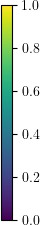
\includegraphics[width=0.06\textwidth]{papers/cahnhilliard/presentation/images/ccb}}
\end{figure}

\subsection{Gegenmassnahmen}
Verwenden wir nun die Integralform der Kontinuitätsgleichung.
Anwenden Reynolds Transporttheorem (wichtiges Resultat der Fluiddynamik)
Zeitableitung bedeutet hier zeitliche Ableitung des Materials.
% TODO: Zitat / Quelle
\begin{align*}
\pderiv{}{t} \int_\Omega c \di{x}
&=
- \int_{\partial\Omega} \flux \cdot n \di{s}
\\
\int_\Omega \pderiv{c}{t} + \nabla \cdot (c v) \di{x}
&=
- \int_{\partial\Omega} \flux \cdot n \di{s}
\end{align*}
Nach anwenden des Divergenztheorems und da Geschwindigkeit divergenzfrei erhalten wir
\begin{align*}
\pderiv{c}{t} + v \cdot \nabla c
&=
\nabla \cdot (M \nabla \mu)
\\
\mu
&=
\deriv{F}{c} -  \epsilon^2 \Delta c
\\
\nabla \cdot v
&=
0
\end{align*}
Zudem beschreiben wir den Einfluss des Rührprozesses über die periodischen Randbedinungen
\begin{alignat*}{2}
v_x(x, y, t)
&=
\alpha \sin(y + \phi_n)
,\quad&
& n \tau \leq t < (n+1) \tau
\\
v_y(x, y, t)
&=
\alpha \sin(x + \psi_n)
,&
& n \tau \leq t < (n+1) \tau
\end{alignat*}
\end{align*}

% TODO: Add plots of stirring process
